%% ****** Start of file aiptemplate.tex ****** %
%%
%%   This file is part of the files in the distribution of AIP substyles for REVTeX4.
%%   Version 4.1 of 9 October 2009.
%%
%
% This is a template for producing documents for use with 
% the REVTEX 4.1 document class and the AIP substyles.
% 
% Copy this file to another name and then work on that file.
% That way, you always have this original template file to use.

%\documentclass[aip,jap,numerical,preprint]{revtex4-1}
\documentclass[twocolumn,secnumarabic,amssymb, nobibnotes, aps, pra]{revtex4}
\newcommand{\revtex}{REV\TeX\ }
\newcommand{\classoption}[1]{\texttt{#1}}
\newcommand{\macro}[1]{\texttt{\textbackslash#1}}
\newcommand{\m}[1]{\macro{#1}}
\newcommand{\env}[1]{\texttt{#1}}
\setlength{\textheight}{9.5in}

\usepackage{amsmath}
\usepackage{graphicx}
\usepackage{booktabs}
\usepackage{color}
\usepackage{enumerate}
\providecommand{\e}[1]{\ensuremath{\times 10^{#1}}}

%\draft % marks overfull lines with a black rule on the right

\begin{document}

%Title of paper
\title{Milikan Oil Drop Experiment
% \large{Methods of experimental physics} \\ 
 %\normalsize{PHYS 413}
 }

% repeat the \author .. \affiliation  etc. as needed
% \email, \thanks, \homepage, \altaffiliation all apply to the current
% author. Explanatory text should go in the []'s, actual e-mail
% address or url should go in the {}'s for \email and \homepage.
% Please use the appropriate macro foreach each type of information

% \affiliation command applies to all authors since the last
% \affiliation command. The \affiliation command should follow the
% other information
% \affiliation can be followed by \email, \homepage, \thanks as well.
\author{Jason Morgan}
%\email[]{Your e-mail address}
%\homepage[]{Your web page}
%\thanks{}
%\altaffiliation{}
\affiliation{Department of Physics, Old Dominion University, Norfolk VA 23529}

%\author{H. Hagood}
%\affiliation{Department of Physics, Old Dominion University, Norfolk VA 23529}


\date{\today}


\begin{abstract}
This experiment determines the charge of an electron by comparing the gravational force on the oil drop to the electromagnetic force on the oil drop.
\end{abstract}

\maketitle
\section{Introduction}

In order to find the charge of the electron, the charge of several electron clusters were measured, then a common factor was calculated. The electron clusters were measured using a Millikan oil drop apparatus. This device suspends a small mist of charged oil droplets within a capacitor and allows an observer to time their movements with or without an electric field. By comparing the gravitational force to the electromagnetic force the complete charge on a single droplet can be measured. After several droplets are observed (and the smallest common denominator determined) the number can be compared to a known value. 

\section{Experimental setup and procedures}

\begin{figure} [h]  %htb stands for here, top and bottom and gives a suggestion to Latex where to place the graph
\begin{center}
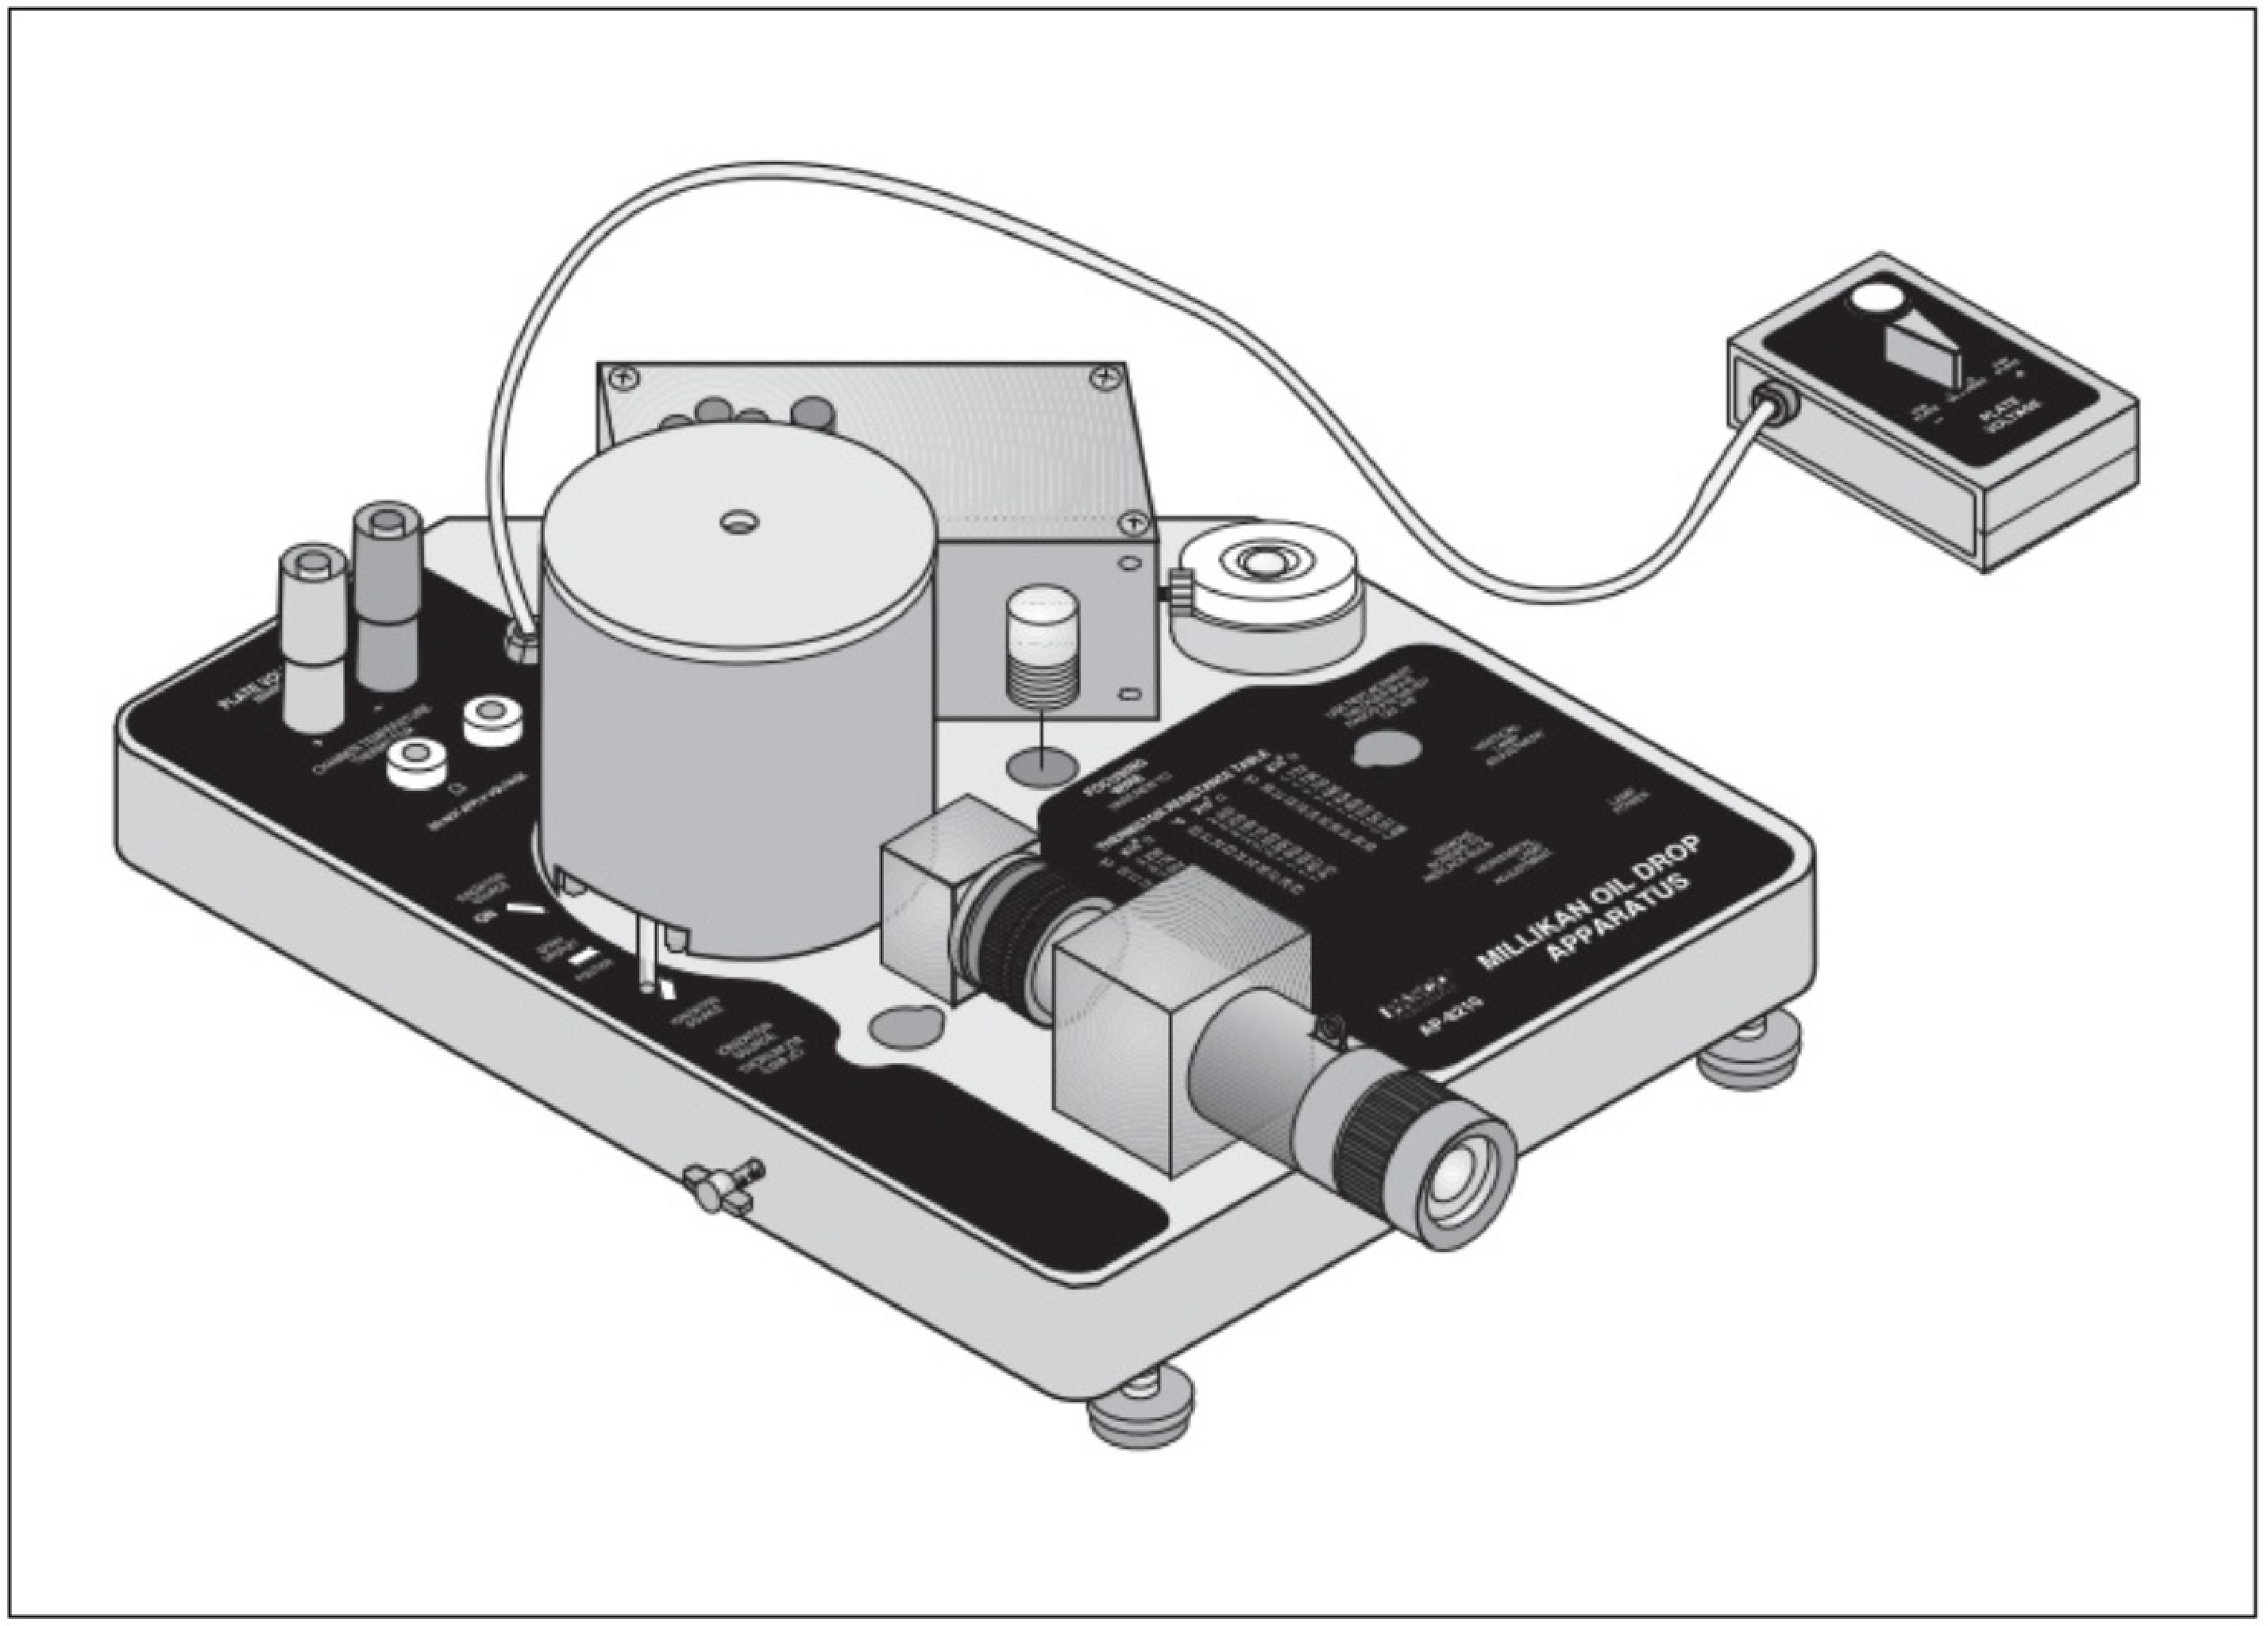
\includegraphics[width=85mm]{setup.pdf} 
\end{center}
\caption{The 'PASCO AP-8210' Millikan Oil Drop Apparatus}
\label{fig:setup}
\end{figure}

The device used in this experiment (the PASCO AP-8210) varies little from Millikan and Fletcher's original design. The chamber into which the oil droplets are sprayed consists of a cylindrical collection area with a small hole in the top just large enough for the tip of the atomizer. At the bottom of the chamber is a diverter which channels the oil mist to a minuscule viewing region. Attached to this region is a horizontal microscope lens, transparent grid, and light source. Above and below the viewing area are the parallel plates of the capacitor (which produce the electric field). Adjacent to the chamber is an ionization source (which supplies the drops with electrons).

\begin{figure} [h] 
\begin{center}
\includegraphics[width=85mm]{setuplabel.eps} 
\end{center}
\caption{Oil Drop Apparatus Components}
\label{fig:label}
\end{figure}

This arrangement is mounted onto a flat base along with wiring for the plates and ionization source, a bull's eye level, and adjustable legs. The apparatus is also equipped with a thermistor in order to accurately gage the air temperature within the chamber (an important variable in air viscosity). Unlike the control for the ionization source, the control for the capacitor is attached via cord so that the frequent switching does not interfere with the drops. Likewise, the whole device is settled on a cushion of sand to minimize vibration transferring through the table. 

To begin, the chamber was cleaned of oil, a small pin was paced in the viewing area and the light source was turned on. By adjusting the microscope and angle of light, the pin was brought into focus and removed. After returning the chamber to order, a continuous mist of oil drops were carefully introduced and the ionization source activated. Once droplets were visible from the viewing lens, the mist was discontinued and the ionization source turned off.

For a brief while the mist was observed to locate an optimal drop. Then the capacitor was alternately turned on and off. As this was done, the drop alternately rose and fell. Each transit was timed and recorded. Eventually, the drop would be lost to the background, measurements would cease and the process repeated. Each individual run of the experiment produced an independent set of data (along with the current values for the capacitor voltage and thermistor). The data was then averaged and the charge for that particular drop was calculated using:

\begin{equation}
q= \frac{4}{3} \pi\rho g\left [ \sqrt{\left ( \frac{b}{2p} \right )^{2}+\frac{9\, \eta \, v_{f}}{2g\rho }} \; -\; \frac{b}{2p}\right ]^{3}\; \frac{v_{f}\: +\: v_{r}}{E\: v_{f}},
%\label{Equation1}  
\end{equation}

where:

\begin{table} [htb]
\begin{tabular}{cl}
$q$ & - total charge ($coulombs$)\\
$d$ & - separation on plates ($m$)\\
$\rho$ & - density of oil ($kg/m^{3}$)\\
$g$ & - acceleration of gravity ($m/s^{2}$)\\
$\eta$ & - viscosity of air ($Ns/m^{2}$)\\
$b$ & - barometric pressure ($Pa-m$)\\
$v_{f}$ & - velocity of falling drop ($m/s$)\\
$v_{r}$ & - velocity of rising drop ($m/s$)\\
$E$ & - voltage/d ,\\
\end{tabular}
\end{table}
which concluded the experiment.


\section{Results and Discussion}

Numerous attempts were made to accurately time the motion of a droplet, three were finally measured with some level of confidence (see Table \ref{tab:tuning}).

\begin{table} [htb]  % Capital letters stronger suggestion
\caption{}      %title of the table     
%\centering              % centering table
\begin{tabular}{cc} % creating four columns (c stands for ceneter, r for right, l for left)
\hline\hline %inserting double-line
Total Charge (coulombs)  & Electrons \\
\hline % inserts single-line
$1.31\e{-19}(\pm$ 4\e{-21}) & 0.82\\
$3.02\e{-19}(\pm$ 2\e{-21}) & 1.88\\
$6.72\e{-19}(\pm$ 1\e{-21}) & 4.19\\

%\hline % inserts single-line
\end{tabular}
\label{tab:tuning}
\end{table}

The smallest charge of the three (which appeared to posses only one excess electron) held a charge of $1.31\e{-19}(\pm$ 4\e{-21}) coulombs, which varies from the expected value of 1.60\e{-19} coulombs by 22\%.

The percent difference from expected values predictably decreased with both the second and third data sets, as the number of electrons increased, giving around 5\% differences. Without knowledge of the accepted value for an electron charge, the third data set would have been calculated as possessing around 5 electrons instead of 4, and the second set would have been calculated at closer to 2.5 electrons (which starkly contradicts quantization).

\section{Conclusion}



Overall, this experiment lacked a degree of rigor. Although most aspects were held in at an acceptable level of control, the human error involved in the timing process and the subjective nature of droplet selection left a significant gap in the scientific process. It is not coincidence that this experiment has historically been criticized by prominent physicists such as Richard Feynman. That said (and despite its inherent flaws), the merit of this experiment is apparent in its continued popularity and the remarkable persistence of its findings. Although this rendition was unable to fully replicate its results, the Millikan Oil Drop remains among the foremost experiments of modern physics.


%Write down references
%-----------------------------------
\begin{thebibliography}{5}
\bibitem{3} Sunny Bishop, \textit{MILLIKAN OIL DROP APPARATUS}, (10101 Foothills Blvd. Roseville, CA).
\bibitem{1} Wikipedia. "Oil drop experiment.", \textit{Wikipedia}, Wikimedia Foundation, 21 April 2014. Web. 22 April 2014.
\bibitem{2} Wikipedia. "Robert Andrews Millikan.", \textit{Wikipedia}, Wikimedia Foundation, 20 April 2014 . Web. 22 April 2014.
\end{thebibliography}

\end{document}

%
% ****** End of file aiptemplate.tex ******
